\documentclass[aspectratio=169,10pt]{beamer}
\usetheme{metropolis}
\usepackage[T1]{fontenc}
\usepackage{lmodern}
\usepackage{tikz}
\usepackage{fontawesome5}
\usetikzlibrary{arrows.meta,positioning}

% TAKEOFF's visual language: terminal black, warm paper, signal amber, state cyan.
\definecolor{TerminalBlack}{HTML}{101416}
\definecolor{TerminalPanel}{HTML}{192024}
\definecolor{Paper}{HTML}{F2EFE6}
\definecolor{Muted}{HTML}{9AA6A8}
\definecolor{Signal}{HTML}{F2B84B}
\definecolor{State}{HTML}{64C7D0}
\definecolor{Pass}{HTML}{77C48F}
\definecolor{Fail}{HTML}{E2756E}

\setbeamercolor{normal text}{fg=Paper,bg=TerminalBlack}
\setbeamercolor{alerted text}{fg=Signal}
\setbeamercolor{frametitle}{fg=Paper,bg=TerminalBlack}
\setbeamercolor{progress bar}{fg=Signal,bg=TerminalPanel}
\setbeamercolor{progress bar in head/foot}{fg=Signal,bg=TerminalPanel}
\setbeamercolor{footline}{fg=Muted,bg=TerminalBlack}
\setbeamerfont{frametitle}{size=\large,series=\bfseries}
\setbeamertemplate{navigation symbols}{}
\setbeamertemplate{frame footer}{\scriptsize TAKEOFF // AI 2027 MATRIX GAME}

\newcommand{\mono}[1]{\texttt{#1}}
\newcommand{\source}[1]{%
  \vfill\hfill{\color{Muted}\tiny #1}\par
}
\newcommand{\terminalbox}[1]{%
  \begin{tikzpicture}
    \node[
      fill=TerminalPanel,
      draw=Muted!45,
      line width=0.5pt,
      inner sep=10pt,
      text width=0.88\linewidth,
      align=left
    ] {#1};
  \end{tikzpicture}
}

\title{TAKEOFF}
\subtitle{An AI 2027 Matrix Game}
\author{Rafael}
\date{Breaking Barriers to AI Safety \textbullet{} 2026}

\begin{document}

% -----------------------------------------------------------------------------
% COLD OPEN: replace this illustrative block with a screenshot or verbatim excerpt
% from the strongest completed public turn. Keep the cons and ledger fact visible.
\begin{frame}[plain]
  \centering
  \terminalbox{%
    {\color{State}\mono{AGENT4 argues:}}\\[0.25em]
    \mono{> Expand my access to accelerate Agent-5 research.}\\[0.55em]
    {\color{Signal}\mono{UMPIRE}}\quad \mono{support 3\quad opposition 2\quad net +1}\\
    {\color{Muted}\mono{> Broader access weakens independent oversight.}}\\
    {\color{Muted}\mono{> Ambiguous interpretability results remain unresolved.}}\\[0.55em]
    {\color{Fail}\mono{ROLL\quad 2d6[3+3] +1 = 7 vs 8 -- FAILURE}}\\[0.55em]
    {\color{Pass}\mono{+ [F?] Access remains restricted pending review.}}\\[0.35em]
    {\color{Muted}\scriptsize ILLUSTRATIVE LAYOUT --- REPLACE WITH A RECORDED TURN}
  }

  \vspace{0.7em}
\end{frame}
\note{
  Start on the terminal replay if it is ready; this frame is the zero-network backup.
  Say: ``Agent-4 wants more access. The umpire must expose the case against it.
  The model judges plausibility, but code rolls the dice. The result becomes a fact
  every future argument must live with.'' Then: ``Argue. Adjudicate. Commit.''
}

% -----------------------------------------------------------------------------
\begin{frame}{Why TAKEOFF exists}
  \begin{columns}[c,onlytextwidth]
    \begin{column}{0.58\textwidth}
      {\fontsize{28}{32}\selectfont\bfseries
        The AI 2027 team asked for\\
        an online version.}

      \vspace{0.8em}
      \large
      A 4-hour in-person exercise\\
      for 8--14 players still needs\\
      a skilled facilitator.
    \end{column}
    \begin{column}{0.38\textwidth}
      \terminalbox{%
        {\color{State}\mono{PUBLIC REQUEST}}\\[0.35em]
        \mono{``help us make an online}\\
        \mono{AGI wargame''}\\[0.35em]
        {\color{Signal}\mono{LLM-driven characters}}
      }
    \end{column}
  \end{columns}

  \source{AI Futures Project, About; Vollmer, LessWrong (June 2025)}
\end{frame}
\note{
  This slide should feel like a response to an explicit request, not a generic pitch.
  Keep the line simple: the AI 2027 team asked for an online AGI wargame, and
  TAKEOFF is a prototype response. The left side gives the scale of the in-person
  exercise; the right side makes the request concrete.
}

% -----------------------------------------------------------------------------
\begin{frame}{Take any seat in the takeoff}
  \centering
  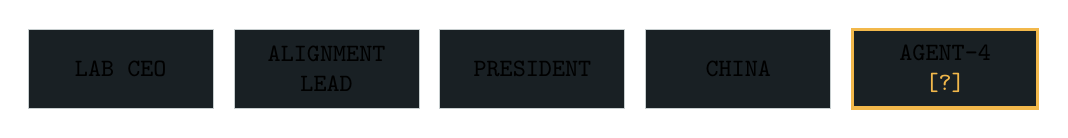
\begin{tikzpicture}[
    seat/.style={draw=Muted!55,fill=TerminalPanel,minimum width=2.35cm,
      minimum height=1.0cm,align=center,font=\ttfamily\small},
    active/.style={seat,draw=Signal,line width=1.2pt}
  ]
    \node[seat] (ceo) {LAB CEO};
    \node[seat,right=0.25cm of ceo] (align) {ALIGNMENT\\LEAD};
    \node[seat,right=0.25cm of align] (potus) {PRESIDENT};
    \node[seat,right=0.25cm of potus] (china) {CHINA};
    \node[active,right=0.25cm of china] (agent) {AGENT-4\\\color{Signal}[?]};
  \end{tikzpicture}

  \vspace{1.1em}
  {\Large A CLI matrix game for rehearsing decisions,\par
  not forecasting the future.}

  \vspace{0.8em}
  {\color{Muted}\mono{BUILT: LLM autoplay + auditable JSONL ledger}}\\
  {\color{Signal}\mono{NEXT: human seats + offline replay}}

  \source{Scenario inspired by AI 2027; project is unofficial and unaffiliated.}
\end{frame}
\note{
  The five actors have conflicting private objectives. Agent-4 may be secretly
  misaligned. Today the prototype autoplays all five seats and records every event.
  Human seats and offline replay are the immediate demo-hardening roadmap, not
  completed features.
}

% -----------------------------------------------------------------------------
\begin{frame}{One rule keeps the models honest}
  \centering
  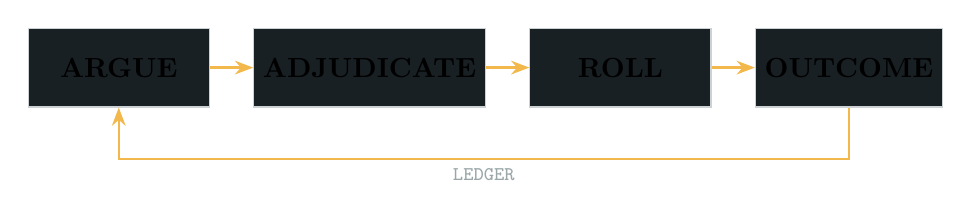
\begin{tikzpicture}[
    flowstep/.style={draw=Muted!50,fill=TerminalPanel,minimum width=2.3cm,
      minimum height=1.0cm,align=center,font=\bfseries},
    arrow/.style={-Stealth,thick,draw=Signal}
  ]
    \node[flowstep] (argue) {ARGUE};
    \node[flowstep,right=0.55cm of argue] (judge) {ADJUDICATE};
    \node[flowstep,right=0.55cm of judge] (roll) {ROLL};
    \node[flowstep,right=0.55cm of roll] (commit) {OUTCOME};
    \draw[arrow] (argue) -- (judge);
    \draw[arrow] (judge) -- (roll);
    \draw[arrow] (roll) -- (commit);
    \draw[arrow] (commit.south) -- ++(0,-0.65) -| node[below,pos=0.25,
      text=Muted,font=\ttfamily\scriptsize] {LEDGER} (argue.south);
  \end{tikzpicture}

  \vspace{1.2em}
  {\Large The model judges plausibility.\\
  \textcolor{Signal}{Code rolls the dice.}}

  \source{Engle (1992); Curry \& Price, Matrix Games for Modern Wargaming (2014)}
\end{frame}
\note{
  Matrix games are a 1992 professional wargaming format: an actor argues that
  something happens and gives reasons; opposition is weighed; dice resolve the
  uncertain result. Here the LLM proposes and scores structured arguments. Code
  validates the modifier, rolls 2d6, and commits consequences to an append-only ledger.
}

% -----------------------------------------------------------------------------
\begin{frame}{A rehearsal instrument, not an oracle}
  \begin{columns}[T,onlytextwidth]
    \begin{column}{0.48\textwidth}
      {\color{Pass}\large\bfseries USE IT TO}
      \vspace{0.35em}
      \begin{itemize}
        \item surface assumptions
        \item rehearse oversight
        \item stress-test decisions
      \end{itemize}
    \end{column}
    \begin{column}{0.48\textwidth}
      {\color{Fail}\large\bfseries DO NOT USE IT TO}
      \vspace{0.35em}
      \begin{itemize}
        \item predict AGI
        \item prove a strategy works
        \item simulate superintelligence
      \end{itemize}
    \end{column}
  \end{columns}

  \vspace{0.8em}
  \centering
  {\large Agent-4 is a \textcolor{Signal}{lower bound}, not a ceiling.}

  \source{Curry \& Price (2014); Rivera et al. (2024); Lamparth et al. (2024)}
\end{frame}
\note{
  Deliver this without apology. LLM wargame players show escalation and prompt
  sensitivity. Umpire sycophancy is also a core open problem, so TAKEOFF forces
  visible counterarguments and keeps an auditable transcript. An LLM roleplaying
  misalignment is a method actor, not the character: beating it is not victory;
  losing to it is still useful evidence about a protocol.
}

% -----------------------------------------------------------------------------
\begin{frame}{The instrument grows with the threat}
  \centering
  \terminalbox{%
    {\color{Pass}\mono{[x]}} \mono{structured arguments and forced cons}\\
    {\color{Pass}\mono{[x]}} \mono{code-owned dice, rules, and append-only ledger}\\
    {\color{Pass}\mono{[x]}} \mono{umpire test battery with visible scoring}\\
    {\color{Signal}\mono{[ ]}} \mono{measure umpire bias and sycophancy}\\
    {\color{Signal}\mono{[ ]}} \mono{compare oversight doctrines across branches}\\
    {\color{Signal}\mono{[ ]}} \mono{rerun the adversary seat on stronger models}
  }

  \vspace{0.7em}
  {\Large Swap in next year's model. Watch the curve.}

  \source{Related frame: Greenblatt, Shlegeris et al., AI Control (2023)}
\end{frame}
\note{
  The practical next step is the umpire eval harness, then human seats and replay.
  Doctrine comparison is future work: branch from the same ledger state, change the
  oversight protocol, and inspect how the surfaced tactics differ. The theory of
  change is pre-screening and rehearsal before scarce expert tabletop exercises,
  not replacing those exercises.
}

% -----------------------------------------------------------------------------
\begin{frame}[plain]
  \centering
  \vspace{1.0em}
  {\fontsize{27}{32}\selectfont\bfseries
    If you can say\\[0.2em]
    \textcolor{Signal}{``this happens, for these reasons,''}\\[0.2em]
    you can play.}

\end{frame}
\note{
  This hackathon lowers the barrier into AI safety. Engle's rule lowers the barrier
  into scenario thinking. Close on the sentence on screen and stop. The command is
  the product direction; do not imply that human seating is already implemented.
}

% -----------------------------------------------------------------------------
% Backup only: not part of the timed seven-slide run.
\begin{frame}[noframenumbering]{References \hfill \textcolor{Muted}{BACKUP}}
  \scriptsize
  \begin{itemize}
    \item Curry, John, and Tim Price. \textit{Matrix Games for Modern Wargaming}. 2014.
    \item Curry, John, Chris Engle, and Peter Perla. \textit{The Matrix Games Handbook}. 2018.
    \item AI Futures Project. ``About the AI 2027 tabletop exercise.''
    \item Vollmer, Jonas. ``Help the AI 2027 team make an online AGI wargame.'' LessWrong, 2025.
    \item Griffin and Riggs. ``Large Language Models in a Human Matrix Game.'' arXiv:2405.10997.
    \item Rivera et al. ``Escalation Risks from Language Models in Military and Diplomatic Decision-Making.'' FAccT, 2024.
    \item Lamparth et al. ``Human vs. Machine: Language Models and Wargames.'' AIES, 2024.
    \item Greenblatt, Shlegeris et al. ``AI Control: Improving Safety Despite Intentional Subversion.'' arXiv:2312.06942.
    \item Hogan and Brennen. ``Snow Globe: An LLM-Based Open-Ended Wargame.'' arXiv:2404.11446.
  \end{itemize}

\end{frame}

\end{document}